% !TeX TS-program = xelatex
\documentclass[twoside=false,DIV=14]{scrartcl}

\usepackage{arev} % order matters, putting this above allows FiraSans to override it for body text
\usepackage[sfdefault]{FiraSans}
\usepackage{inconsolata}
%\usepackage[fira]{fontsetup}
\usepackage{scrlayer-scrpage}
\renewcommand{\titlepagestyle}{scrheadings}
\usepackage{graphicx}
\usepackage{blindtext}
\usepackage{wrapfig}
\usepackage{tabularx}
\usepackage{hyperref}
\usepackage{listings}
\usepackage{tikz}
\usepackage{amsmath}
\usepackage[many]{tcolorbox}

\usepackage{xcolor,sectsty}
\definecolor{blackish}{RGB}{56,58,54}
\definecolor{redish}{RGB}{109,41,49}
\definecolor{red}{RGB}{152,41,50}
\definecolor{orangeish}{RGB}{188,71,0}
\definecolor{blueish}{RGB}{25,33,139}
\subsubsectionfont{\color{blackish}}
\subsectionfont{\color{blackish}}
\sectionfont{\color{blackish}}

\lohead{\color{red} COMP3000 Programming Languages}
\rohead{
\includegraphics[width=0.5cm]{../logo.jpg}}

\setkomafont{author}{\sffamily \small}
\setkomafont{date}{\sffamily \small}

\DeclareOldFontCommand{\bf}{\normalfont\bfseries}{\mathbf}
\DeclareOldFontCommand{\tt}{\normalfont\ttfamily}{\texttt}

\lstset{basicstyle=\ttfamily}


\date{}
\newtcolorbox{aside}[1][]{
  title=Aside,
  width=0.3\textwidth,
  fonttitle=\bfseries,
  breakable,
  fonttitle=\bfseries\color{black},
  colframe=blueish!80,
  colback=blueish!2
  #1}

\newtcolorbox{note}[1][]{
  title=Note,
  width=\textwidth,
  fonttitle=\bfseries,
  breakable,
  fonttitle=\bfseries\color{black},
  colframe=orangeish!80,
  colback=orangeish!2
  #1}

\newtcolorbox{hint}[1][]{
    title=Hint,
    width=\textwidth,
    fonttitle=\bfseries,
    breakable,
    fonttitle=\bfseries\color{white},
    colframe=blueish!80,
    colback=blueish!2
    #1}

\newtcolorbox{todo}[1][]{
  title=!! TODO !!,
  width=\textwidth,
  fonttitle=\bfseries,
  breakable,
  fonttitle=\bfseries\color{white},
  colframe=red!80,
  colback=red!2
  #1}
  
\providecommand{\tightlist}{%
  \setlength{\itemsep}{0pt}\setlength{\parskip}{0pt}}


\title{\color{redish} \vspace{-2em}Week 7 Workshop: Binary Search Trees}

\begin{document}
{\color{blackish}\maketitle}\vspace{-2em}%\input{proposal.inc}
\begin{itemize}
    \item[$\cdot$] {\bf Resources:}  Week 6  Code Bundle.
    \item[$\cdot$] {\bf To submit this week's work:} Submit your solution to Exercise \ref{sec:submission} to your teacher in class.  You should hand in a single piece of paper with your solution on it.  Be sure you include your name, student number, and the week number in the top-right of your submission.
\end{itemize}

\part*{Exercises}

\section{Binary Search Tree: Shape}
This question relates to a binary search tree storing characters.  In lectures we worked with a binary search tree storing integers, but I am sure you can make the generalisation.

Arrange nodes that contain the letters A, C, E, F, L,
V and Z into two binary search trees, one with maximum height and one
that has minimum height.  You can insert those values in any order you wish. Show both final trees and for each give the order of insertion that gave the tree.


\section{Binary Search Tree: Examples}
\label{sec:submission}
Beginning with the indicated binary search tree, draw the binary search trees which are formed when you insert the following values in the order given?  Use the insertion algorithm given in lectures.

\begin{enumerate}
\item  initial tree: W.  insert T, N, J, E, B, A
\item  initial tree: W.  insert T, N, A, B, E, J
\item  initial tree: A.  insert B, W, J, N, T, E
\end{enumerate}

\section{Binary Search Tree: Traversal}
For each tree in question \ref{sec:submission} write down the sequence of letters obtained with an inorder, preorder and postorder traversal.

\section{Binary Search Tree: Deletion}
Use the deletion function given in lectures to redraw the tree after deleting the following letters.  First delete {\tt i}, then {\tt f}, then {\tt a}.  Draw the resulting tree after each deletion.

\begin{verbatim}
        f
      /   \
     c      i
    / \    / \
   b   e   g  w
  /   /      / \
 a   d      m   z 
\end{verbatim}


\section{Binary Search Tree Code: Path}
In a binary tree, a path between the root node and one of its descendants is the list of arcs connecting the two.  If we write $l$ for the left arc and $r$ for the right arc then a path can be described as a string of $l$'s and $r$'s.  For example in the tree

\begin{verbatim}
           7
         /   \
       4      12
     /  \    /  \
   2    6   10   17
  /    /   / \
 1    5   9  11
\end{verbatim}

the path connecting 7 to 10  is $rl$, and the path connecting the 7 to 5 is $lrl$. Using the class code  provided in the bundle, given a target value, implement the function {\tt generatePath} which returns the path from the root to the target value.  Return the path as a String of ls and rs.

If the target value is not in the tree, the function should return the path to the empty slot in which that value would be added and an exclamation point.  For example, \verb+generateString(8)+ should give \verb+rll!+.

\begin{verbatim}
	public String generatePath(int target);
\end{verbatim}

\newpage\setcounter{section}{0}
\part*{Solutions}

\section{Binary Search Tree: Shape}
\begin{note}
There are multiple correct answers to this question for the maximum height, but only one correct tree for the minimum height (though there are multiple insertion orders to get that tree).
\end{note}

Insertion order "ACEFLVZ" gives 
\begin{center}
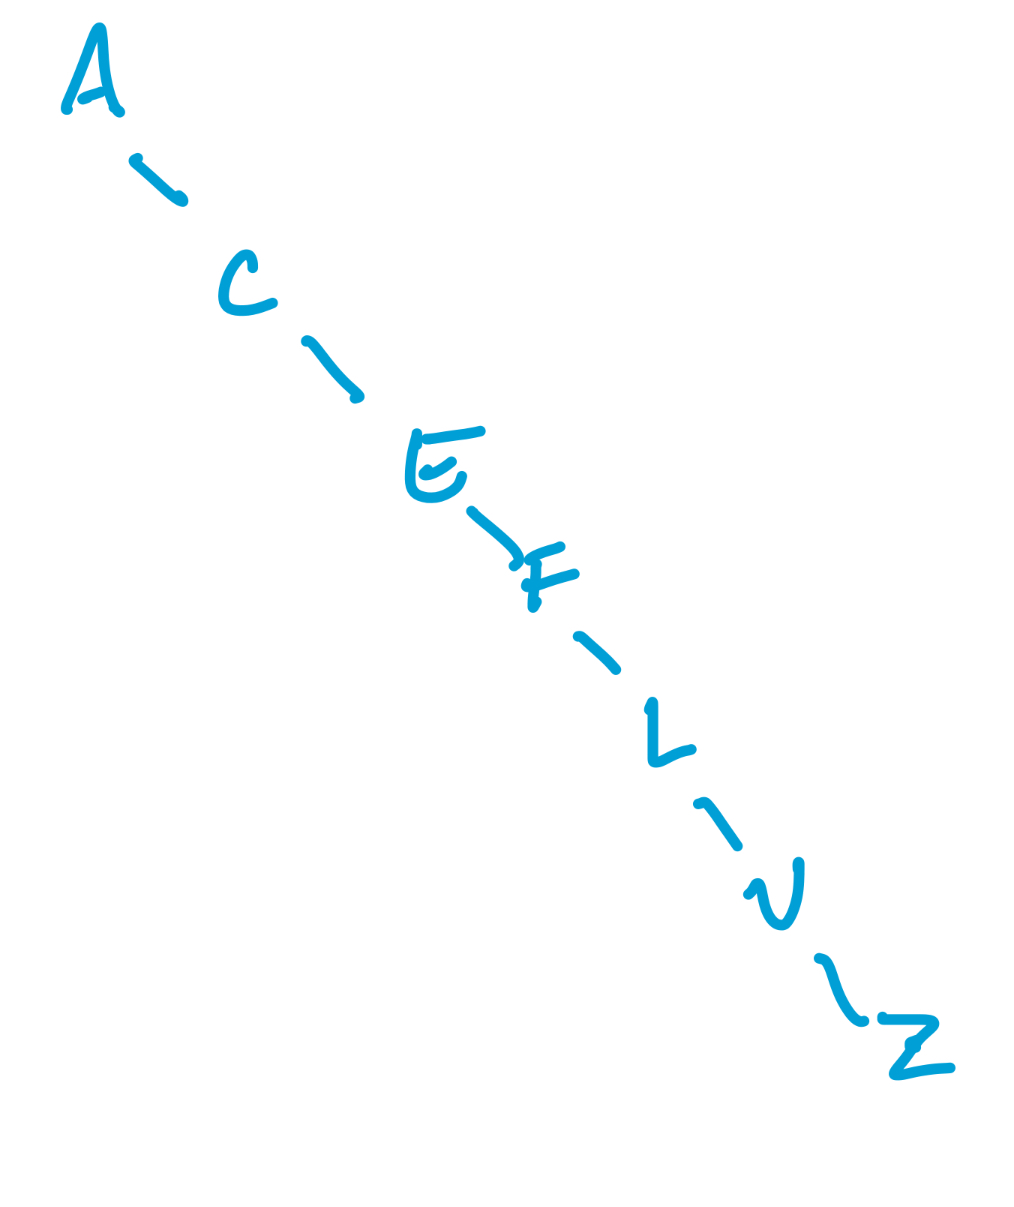
\includegraphics[width=0.3\textwidth]{max_height.jpeg}
\end{center}

Insertion order "FCAEVLZ" gives
\begin{center}
 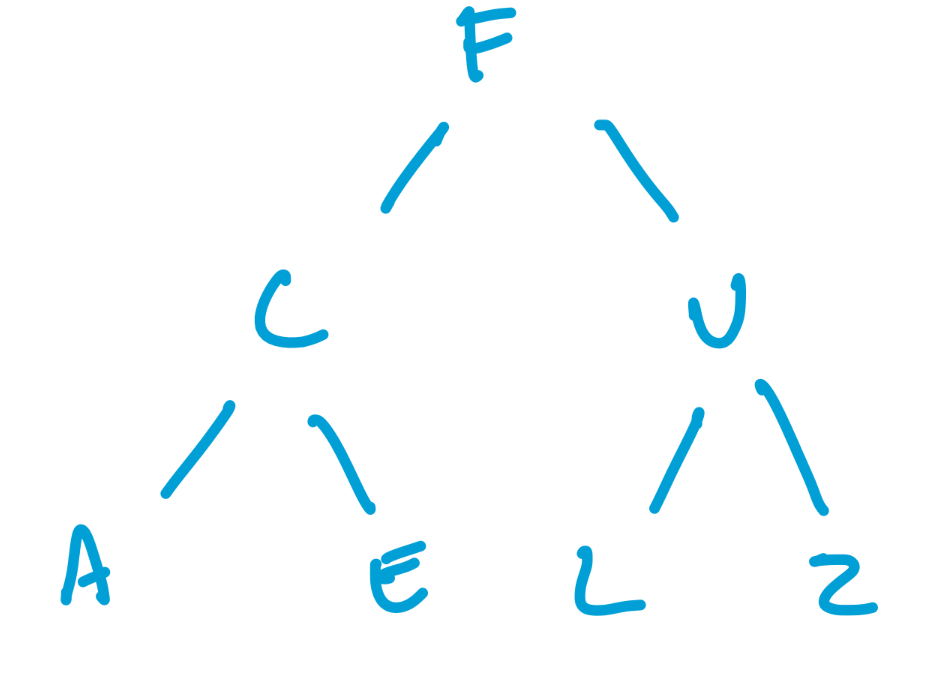
\includegraphics[width=0.4\textwidth]{min_height.jpeg}
 \end{center}

\section{Binary Search Tree: Examples}
\subsection{WTNJEBA}
\begin{center}
  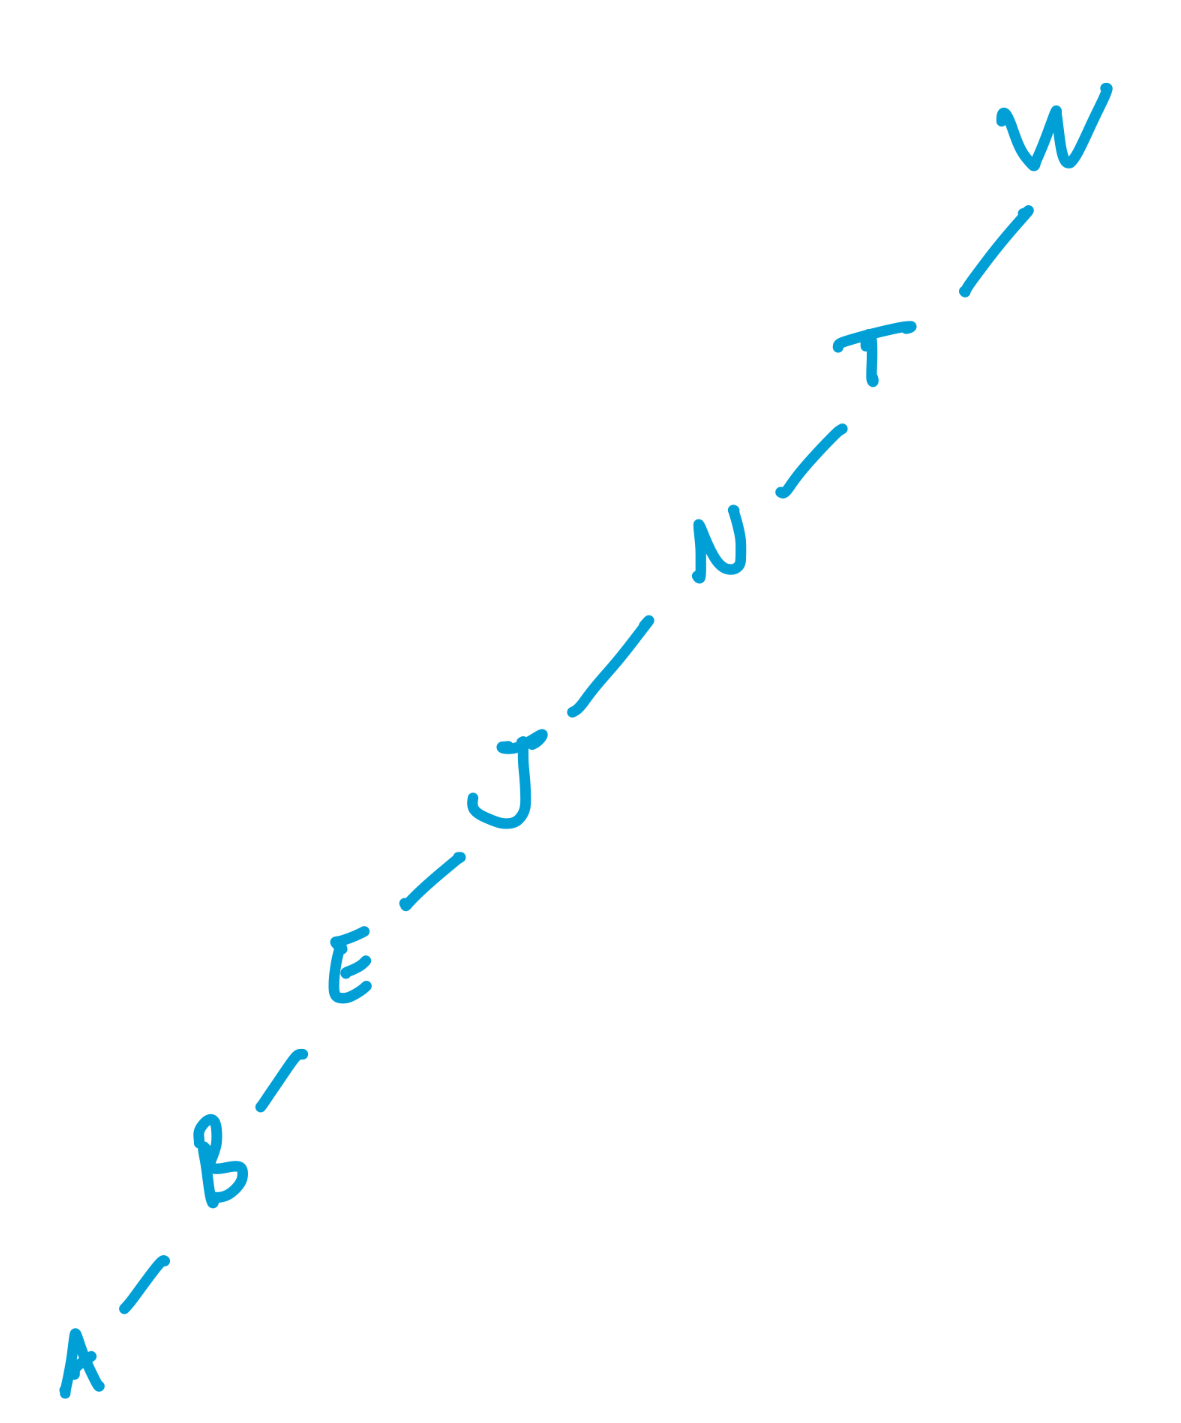
\includegraphics[width=0.3\textwidth]{2_1.jpeg}
  \end{center}
 
\subsection{WTNABEJ}
\begin{center}
  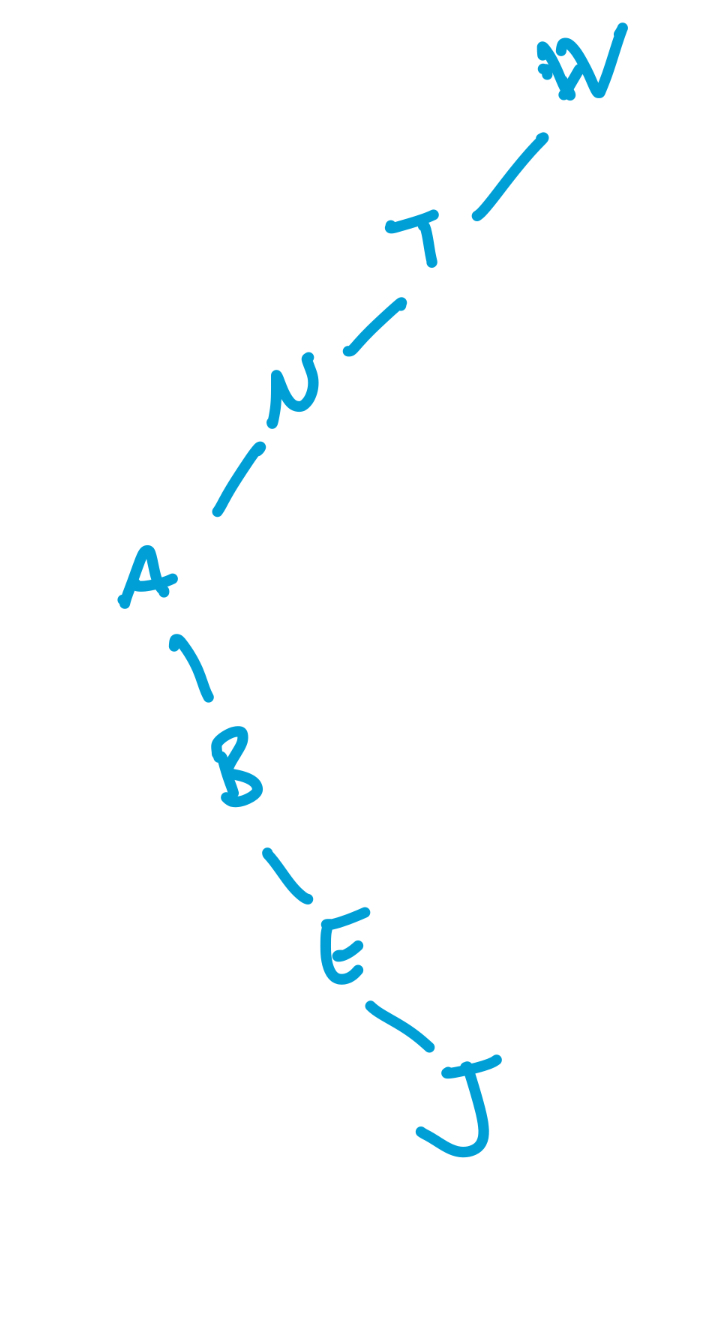
\includegraphics[width=0.3\textwidth]{2_2.jpeg}
  \end{center}
 
\subsection{ABWJNTE}
\begin{center}
  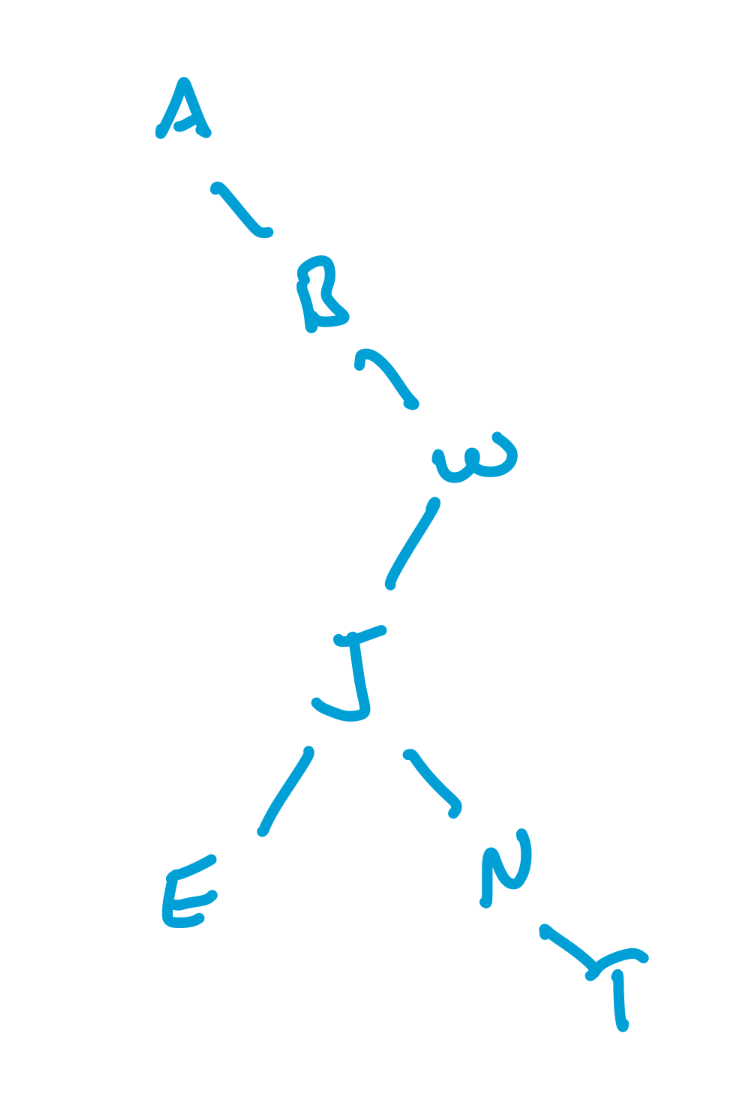
\includegraphics[width=0.3\textwidth]{2_3.jpeg}
  \end{center}
 
\section{Traversal}
\subsection{WTNJEBA}
\begin{description}
\item [preorder] WTNJEBA
\item [inorder] ABEJNTW
\item [postorder]ABEJNTW
\end{description}

\subsection{WTNABEJ}
\begin{description}
\item [preorder] WTNJEBA
\item [inorder] ABEJNTW
\item [postorder]ABEJNTW
\end{description}

\subsection{ABWJNTE}
\begin{description}
\item [preorder] ABWJENT
\item [inorder] ABEJNTW
\item [postorder] ETNJWBA
\end{description}

\section{Binary Search Tree: Deletion}
Here is my trace of each deletion one by one.  The orange (final) tree is the final result of all three deletions.  Note, just like the code we use in lectures, we choose the \emph{greatest value on the left} to be the replacement\footnote{recall that other algorithms might choose the least value on the right.}

\begin{center}
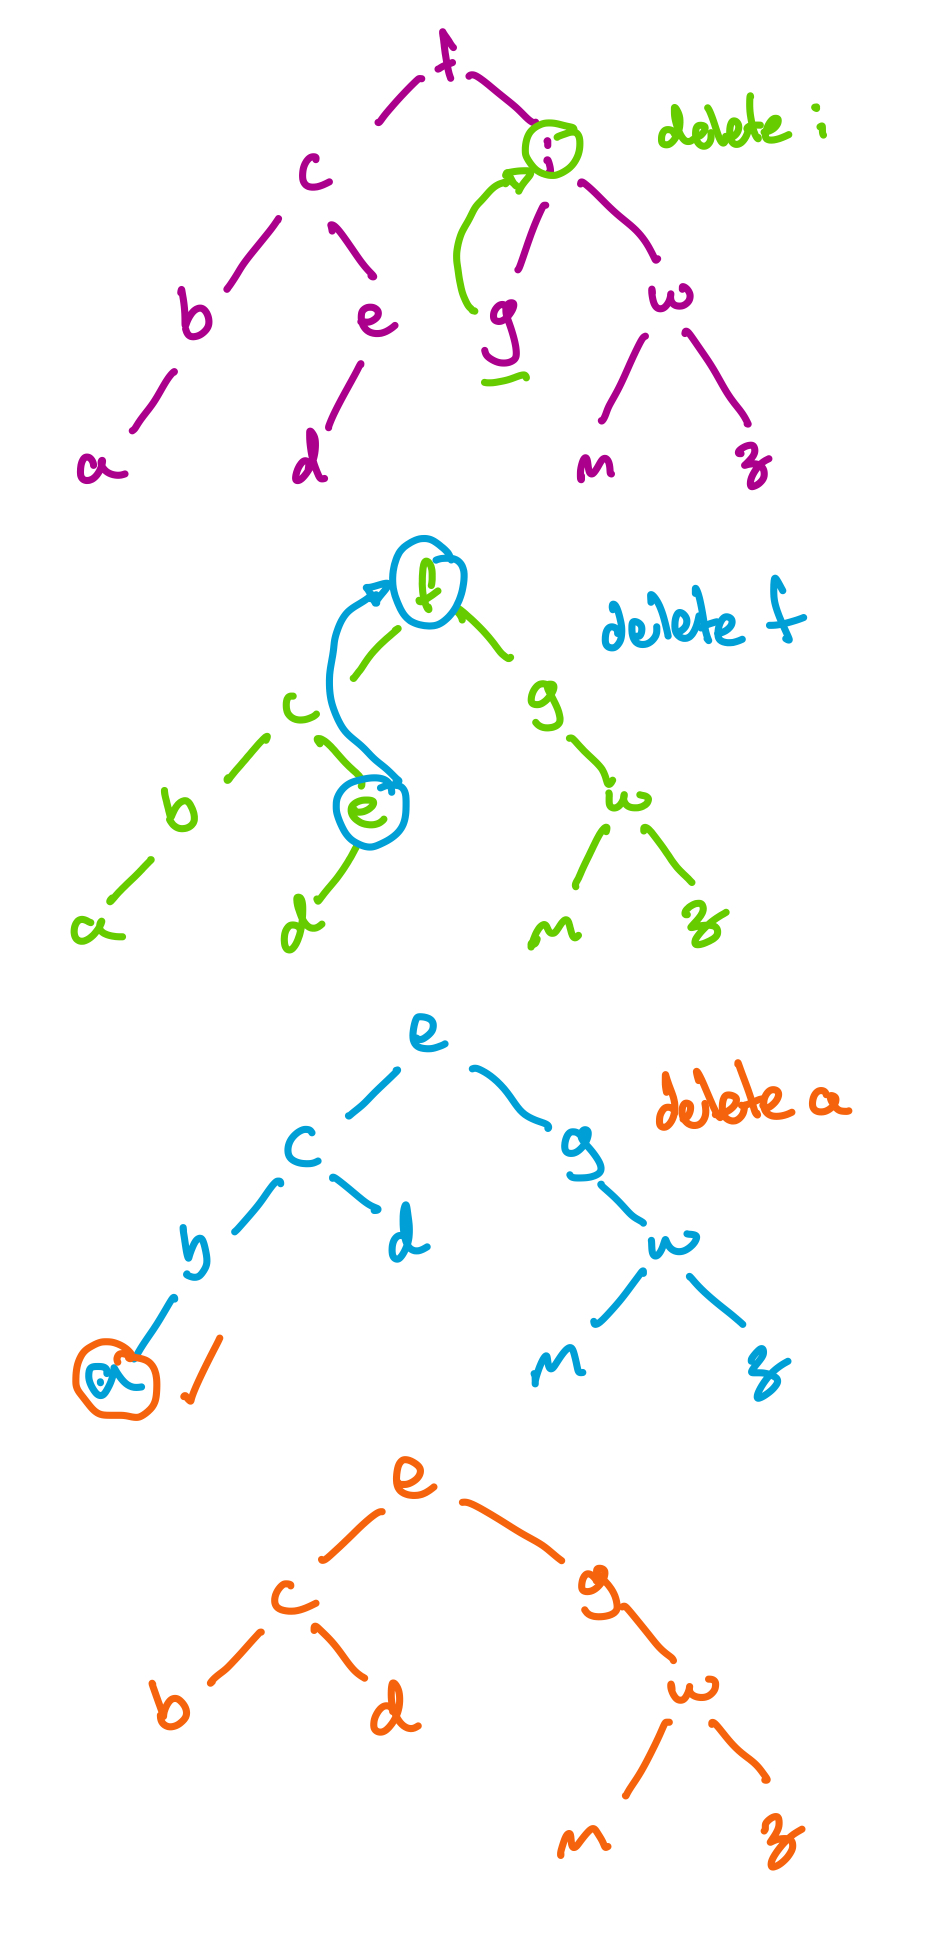
\includegraphics[width=0.5\textwidth]{deletion.jpeg}
\end{center}

\section{Binary Search Tree: Path}
\begin{lstlisting}[language=java]
public String generatePath(int target){
    if (value == target){
        return "";
    } else if (value < target){
        return (right == null)? "!": "r" + right.generatePath(target);
    } else {
        return (left == null)? "!": "l" + left.generatePath(target);
    }
}

@Test
public void testPath(){
    BinarySearchTree ex = new BinarySearchTree(7, null, null);
    ex.insert(4);
    ex.insert(2);
    ex.insert(6);
    ex.insert(1);
    ex.insert(5);
    ex.insert(12);
    ex.insert(10);
    ex.insert(17);
    ex.insert(9);
    ex.insert(11);
    assertEquals(ex.generatePath(10), "rl");
    assertEquals(ex.generatePath(5), "lrl");
    assertEquals(ex.generatePath(17), "rr");
    assertEquals(ex.generatePath(8), "rll!");
}

\end{lstlisting}
\newpage\setcounter{section}{0}
\part*{Self Study}

\section{Binary Search Tree Code: Parts of Tree}
First, write method on a binary search tree which takes two items \verb+a+, \verb+b+
with \verb+a <= b+, and returns a new Binary Search Tree containing all the elements having values lying between \verb+a+ and \verb+b+.
\begin{lstlisting}
static BinarySearchTree treeBetween(int a, int b)
// PRE: a <= b
// POST: Returns a new tree with all the values between a and b
\end{lstlisting}

\section{Binary Search Tree Code: Iterative Insertion}
Write an iterative version of \verb+insert+.

\section{Binary Tree: Practice}
Using the algorithms from lectures, show the tree that results from the insertions given the particular start tree
\begin{enumerate}
\item initial tree: $7$ insert $1,2,3,4,5,6,7,8,9,10$
\item initial tree: $7$ insert $9,8,7,6,5,4,3,2,1,0$
\item initial tree: $7$ insert $0,9,2,8,3,7,4,6,5,1$
\item initial tree: $3$ insert $1,2,3,4,5,6,7,8,9,10$
\item initial tree: $3$ insert $9,8,7,6,5,4,3,2,1,0$
\item initial tree: $3$ insert $0,9,2,8,3,7,4,6,5,1$
\item initial tree: $5$ insert $3,7,2,4,6,10,9,11$
\end{enumerate}
Show the trees that result from \emph{removing} 5 from each of the above trees.

\newpage\setcounter{section}{0}
\part*{Self Study Solutions}

\section{Binary Search Tree Code: Parts of Tree}
{\small
\begin{lstlisting}[language=java]
  BinarySearchTree treeBetween(int a, int b){
    if (a < value && b > value){
       BinarySearchTree fromLeft = (left == null)? null: left.treeBetween(a,b);
       BinarySearchTree fromRight = (right == null)? null: right.treeBetween(a, b);
       return new BinarySearchTree(value, fromLeft, fromRight);
    } else if (a < value){
        return (left == null)? null: left.treeBetween(a, b);
    } else if (b > value){
        return (right == null)? null: right.treeBetween(a, b);
    } else {
        return null;
    }
}

@Test
public void testTreeBetween(){
    BinarySearchTree ex = new BinarySearchTree(7, null, null);
    ex.insert(4);
    ex.insert(2);
    ex.insert(6);
    ex.insert(1);
    ex.insert(5);
    ex.insert(12);
    ex.insert(10);
    ex.insert(17);
    ex.insert(9);
    ex.insert(11);
    assertEquals(ex.treeBetween(4,7).inorder(), "[5][6]");
    assertEquals(ex.treeBetween(4,13).inorder(), "[5][6][7][9][10][11][12]");
}
\end{lstlisting}
}
{\small
\section{Binary Search Tree: Iterative Insertion}
\begin{lstlisting}[language=java]
void insertIterative(int newvalue){
    BinarySearchTree curr = this;
    while (curr != null){
        if (curr.value >= newvalue){
            if (curr.left == null){
                curr.left = new BinarySearchTree(newvalue, null, null);
                return;
            } else {
                curr = curr.left;
            }
        } else {
            if (curr.right == null){
                curr.right = new BinarySearchTree(newvalue, null, null);
                return;
            } else {
                curr = curr.right;
            }
        }
    }
}

@Test
public void testBasicsIterative(){
    BinarySearchTree ex = new BinarySearchTree(4, null, null);
    ex.insertIterative(2);
    ex.insertIterative(5);
    assertEquals(ex.inorder(), "[2][4][5]");
    ex.insertIterative(8);
    ex.insertIterative(1);
    assertEquals(ex.inorder(), "[1][2][4][5][8]");
} 
\end{lstlisting}
}

\section{Binary Tree: Practice}
\begin{tabular}[t]{lcc}
\textbf{insertion order} &  \textbf{tree from insertion} & \textbf{tree after removal of 5} \\
1 & 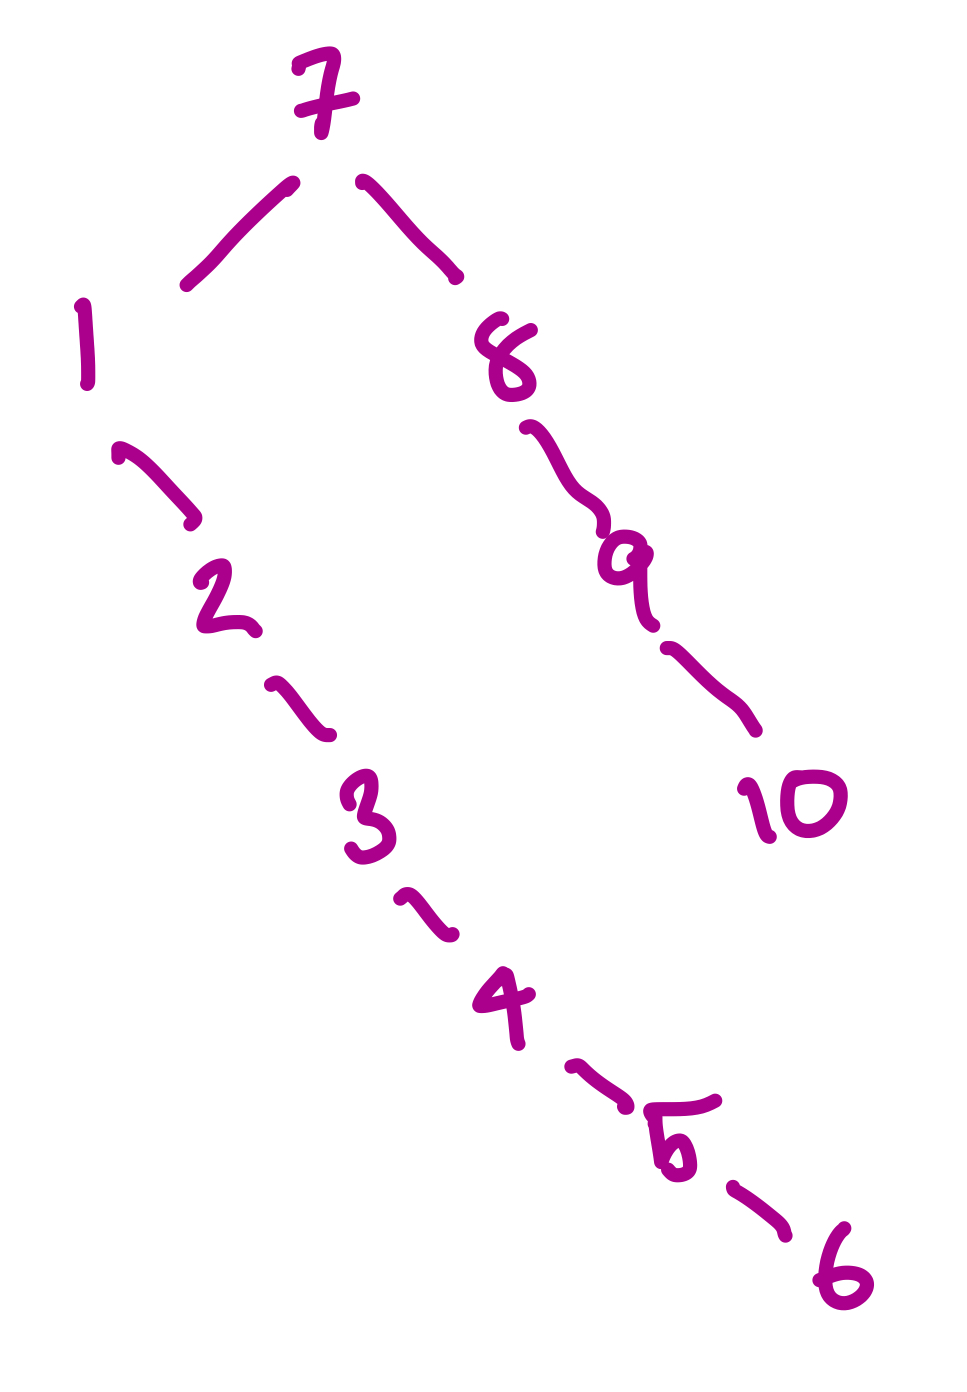
\includegraphics[width=0.3\textwidth]{3_1.jpeg} & 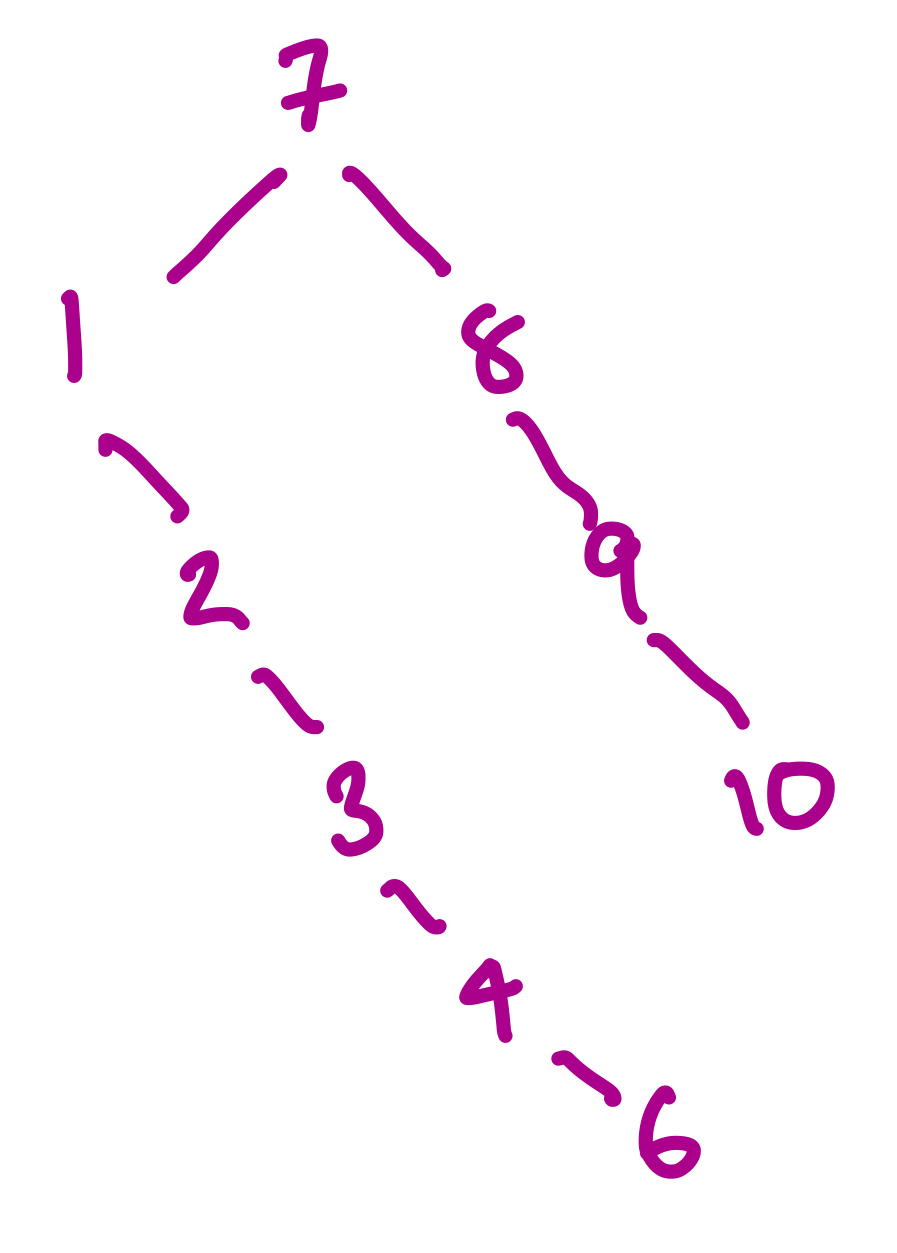
\includegraphics[width=0.3\textwidth]{3_1_removed.jpeg} \\
2 & 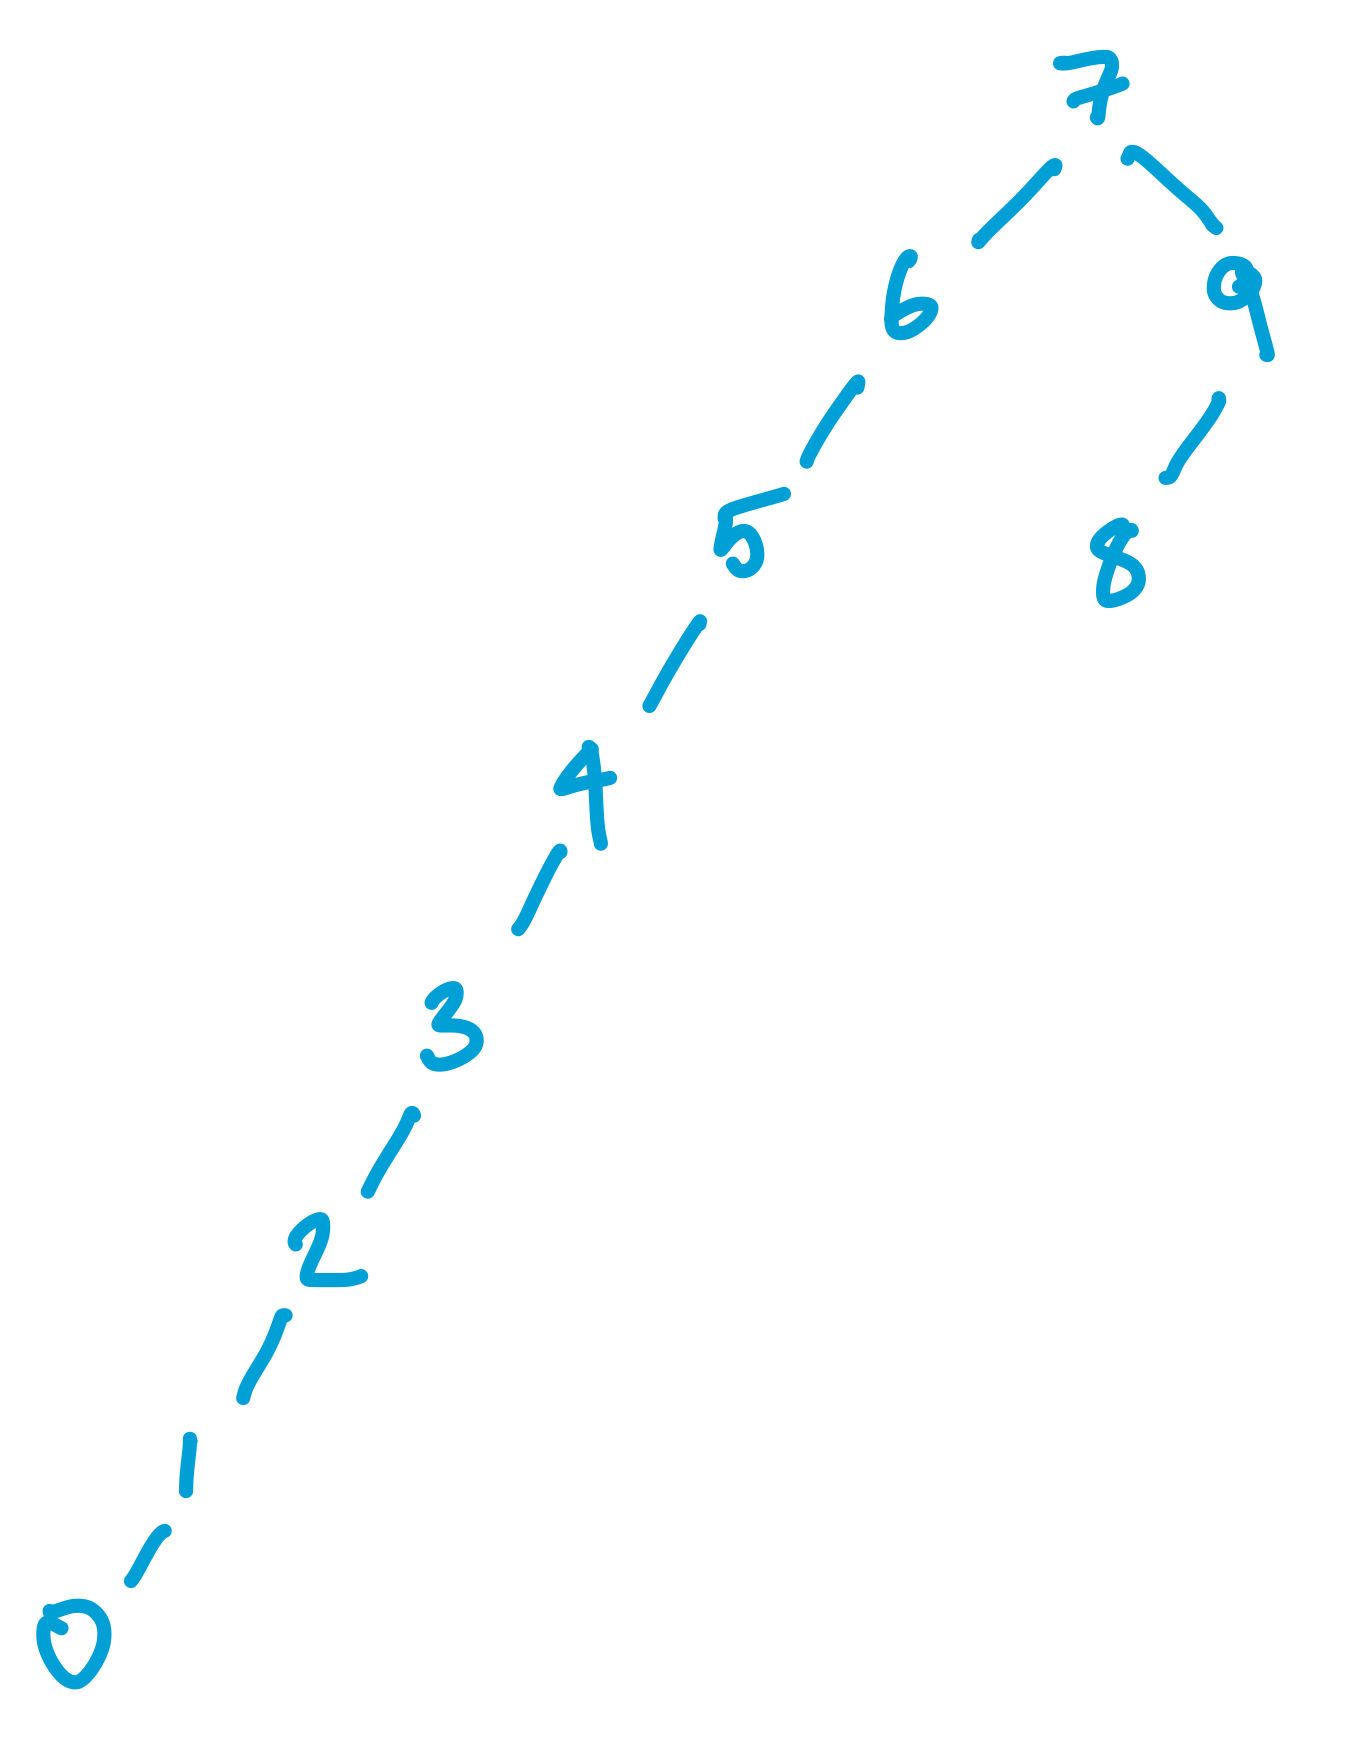
\includegraphics[width=0.3\textwidth]{3_2.jpeg} & 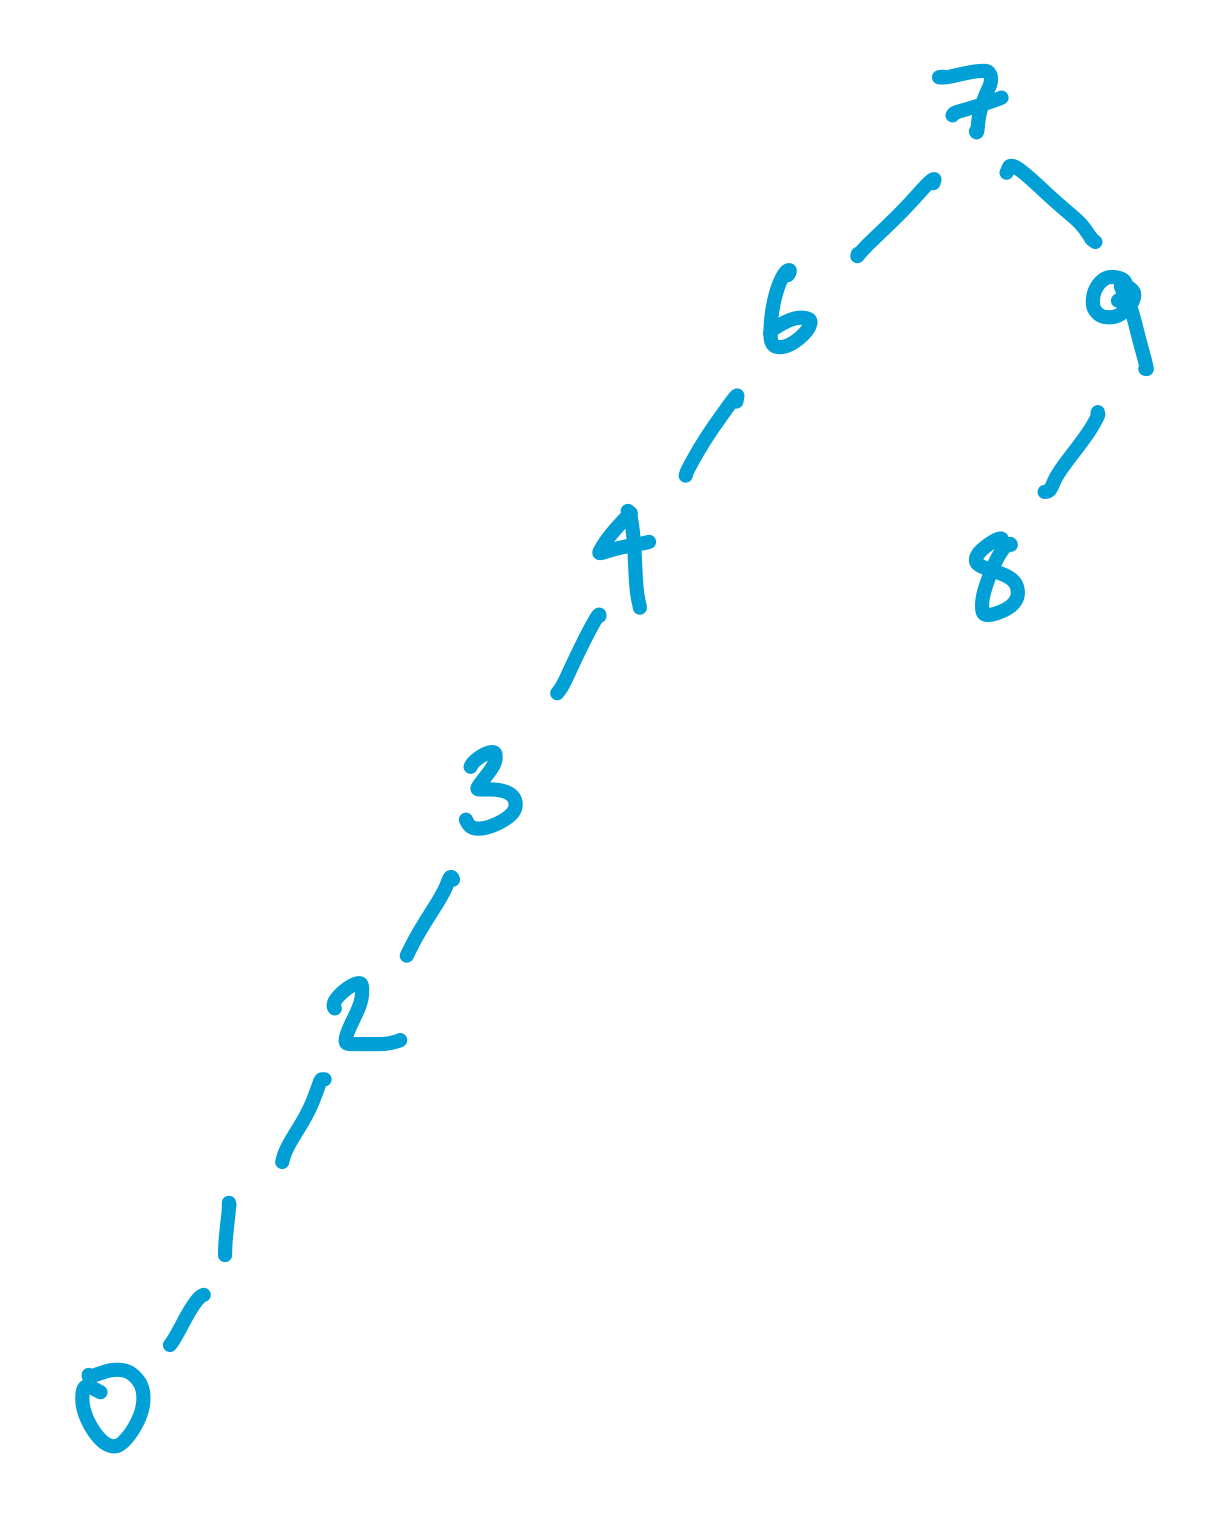
\includegraphics[width=0.3\textwidth]{3_2_removed.jpeg} \\
\end{tabular}

\begin{tabular}[t]{lcc}
  \textbf{insertion order} &  \textbf{tree from insertion} & \textbf{tree after removal of 5} \\
3 & 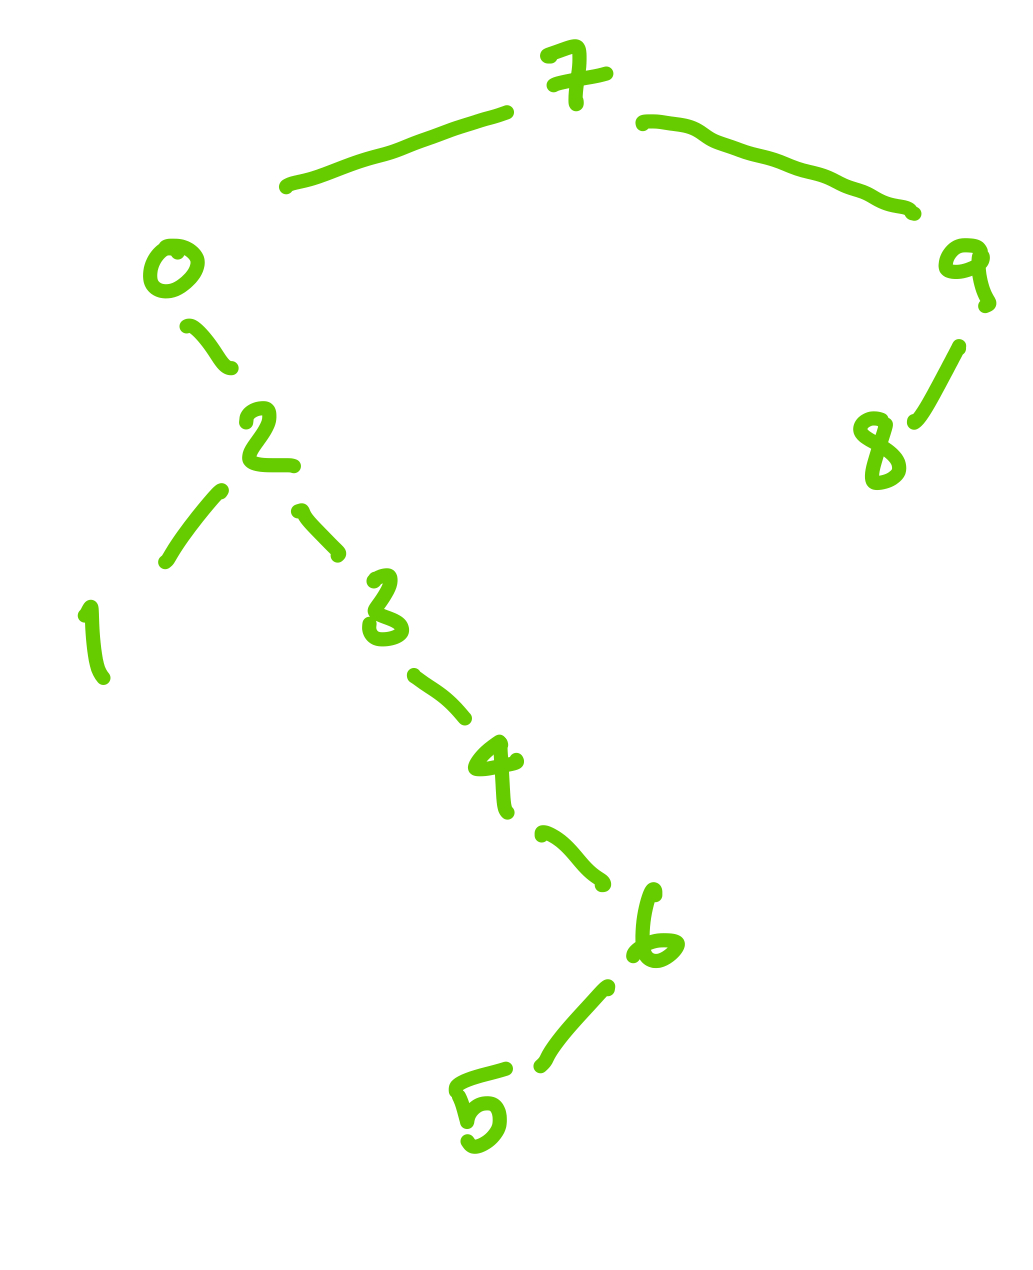
\includegraphics[width=0.3\textwidth]{3_3.jpeg} & 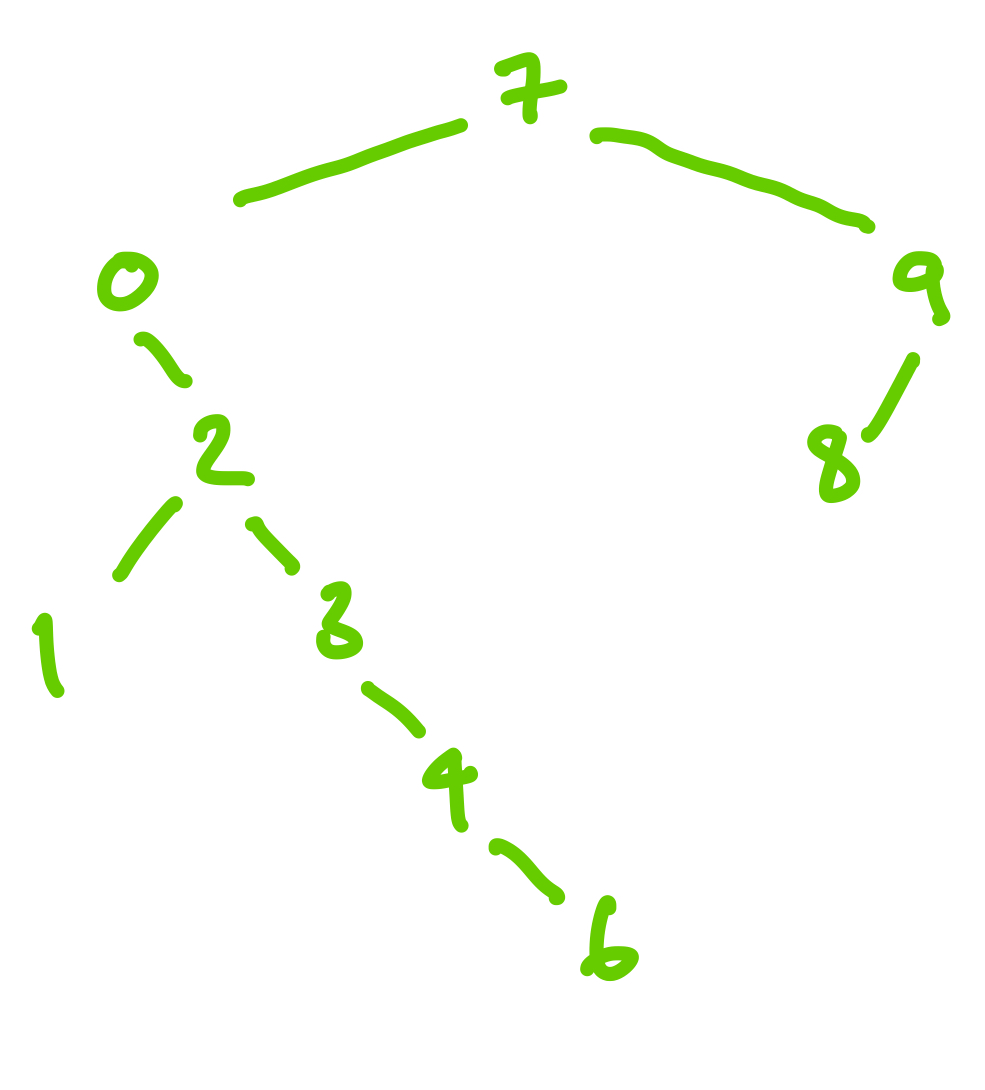
\includegraphics[width=0.3\textwidth]{3_3_removed.jpeg} \\
4 & 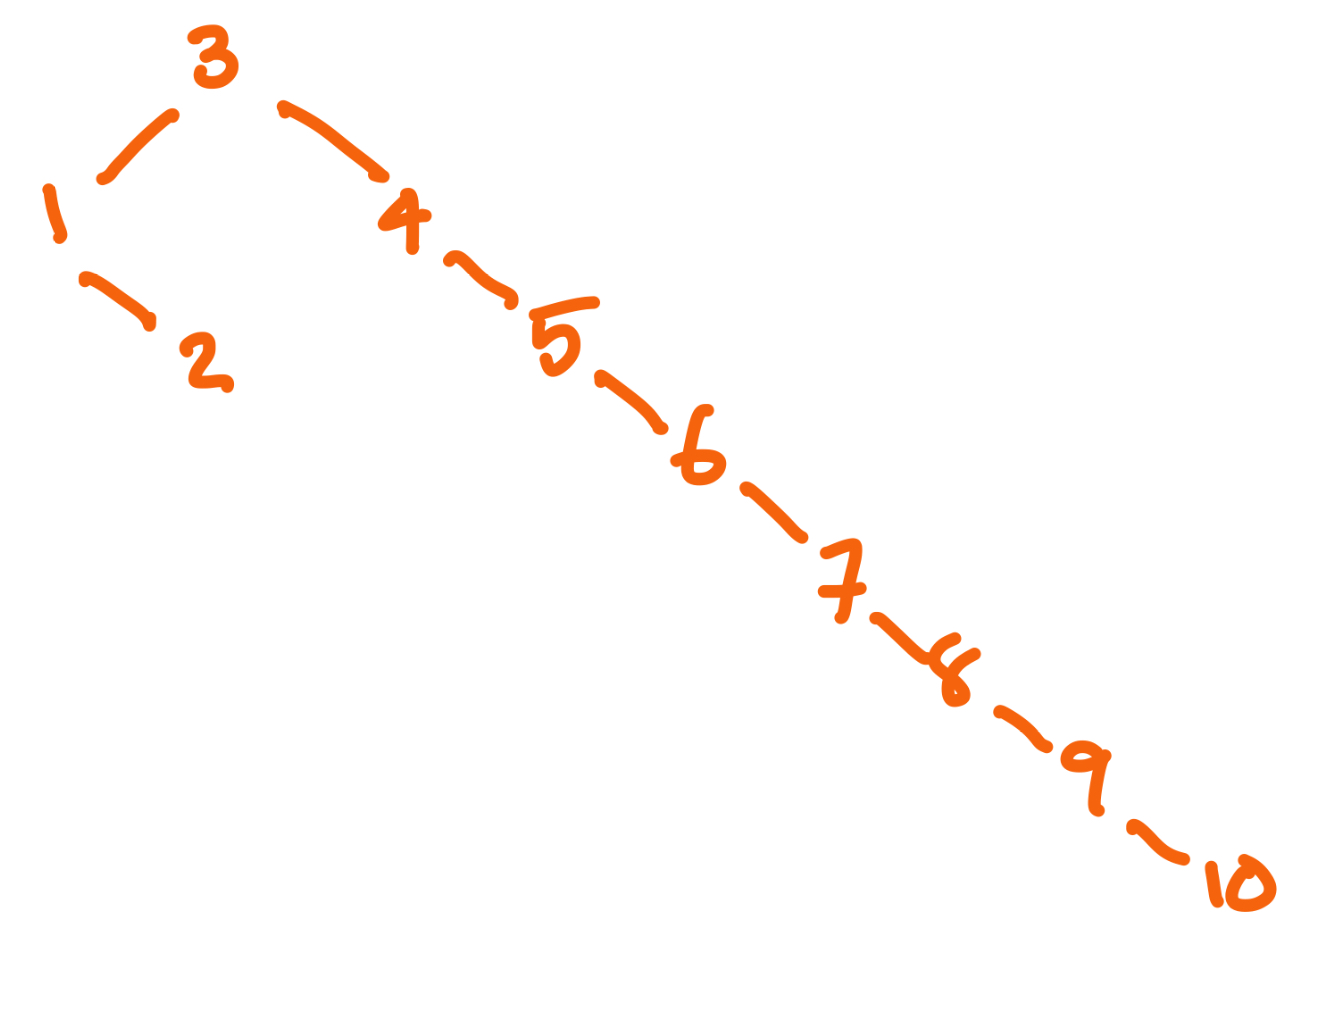
\includegraphics[width=0.3\textwidth]{3_4.jpeg} & 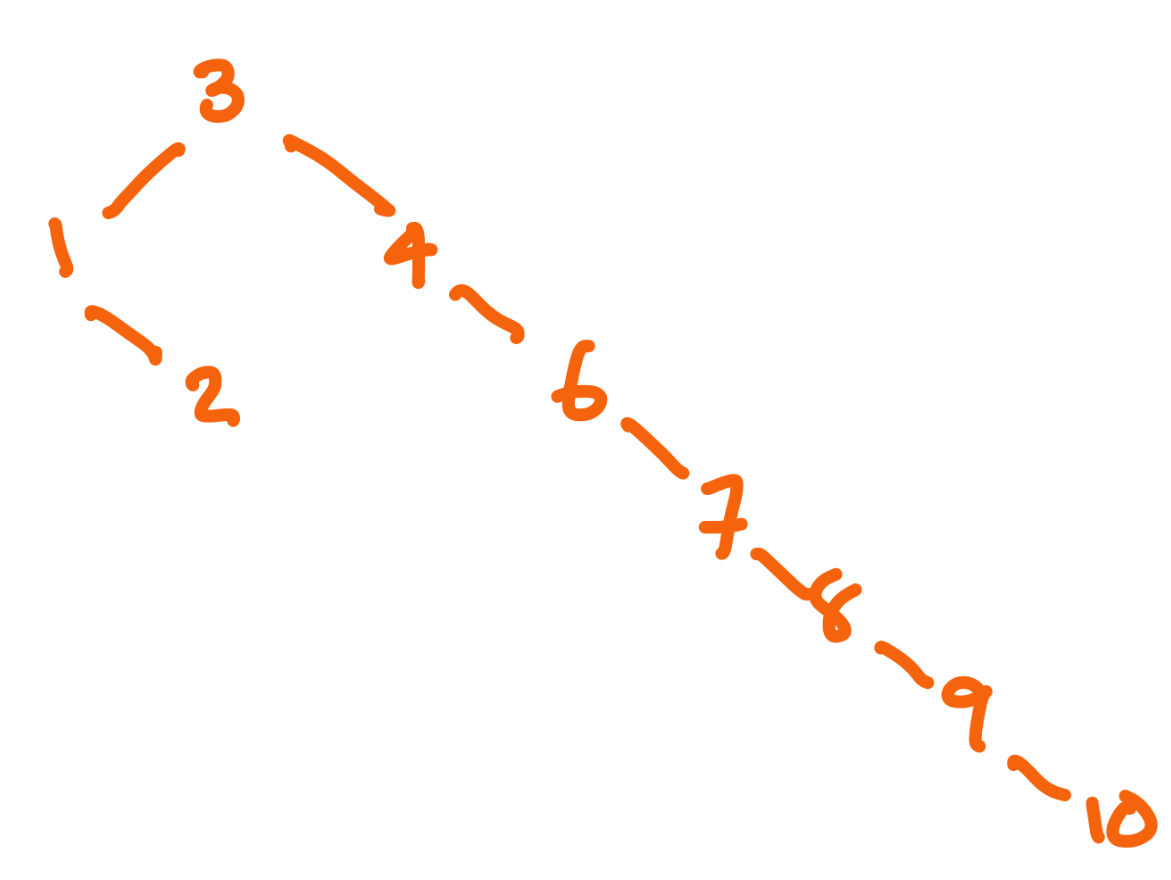
\includegraphics[width=0.3\textwidth]{3_4_removed.jpeg} \\
5 & 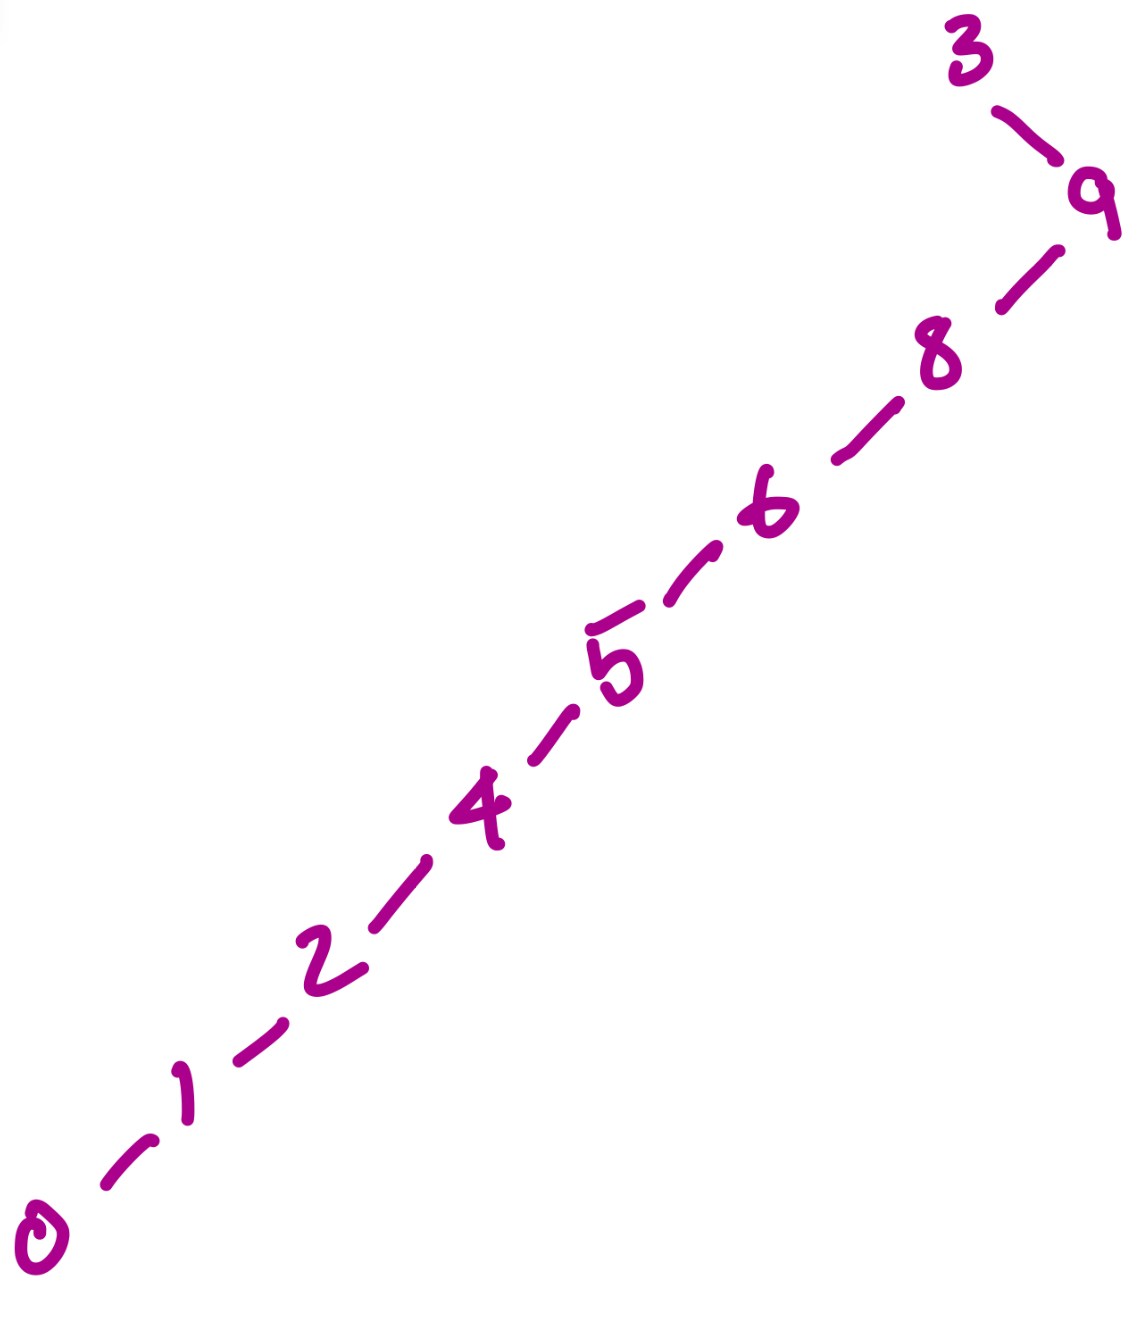
\includegraphics[width=0.3\textwidth]{3_5.jpeg} & 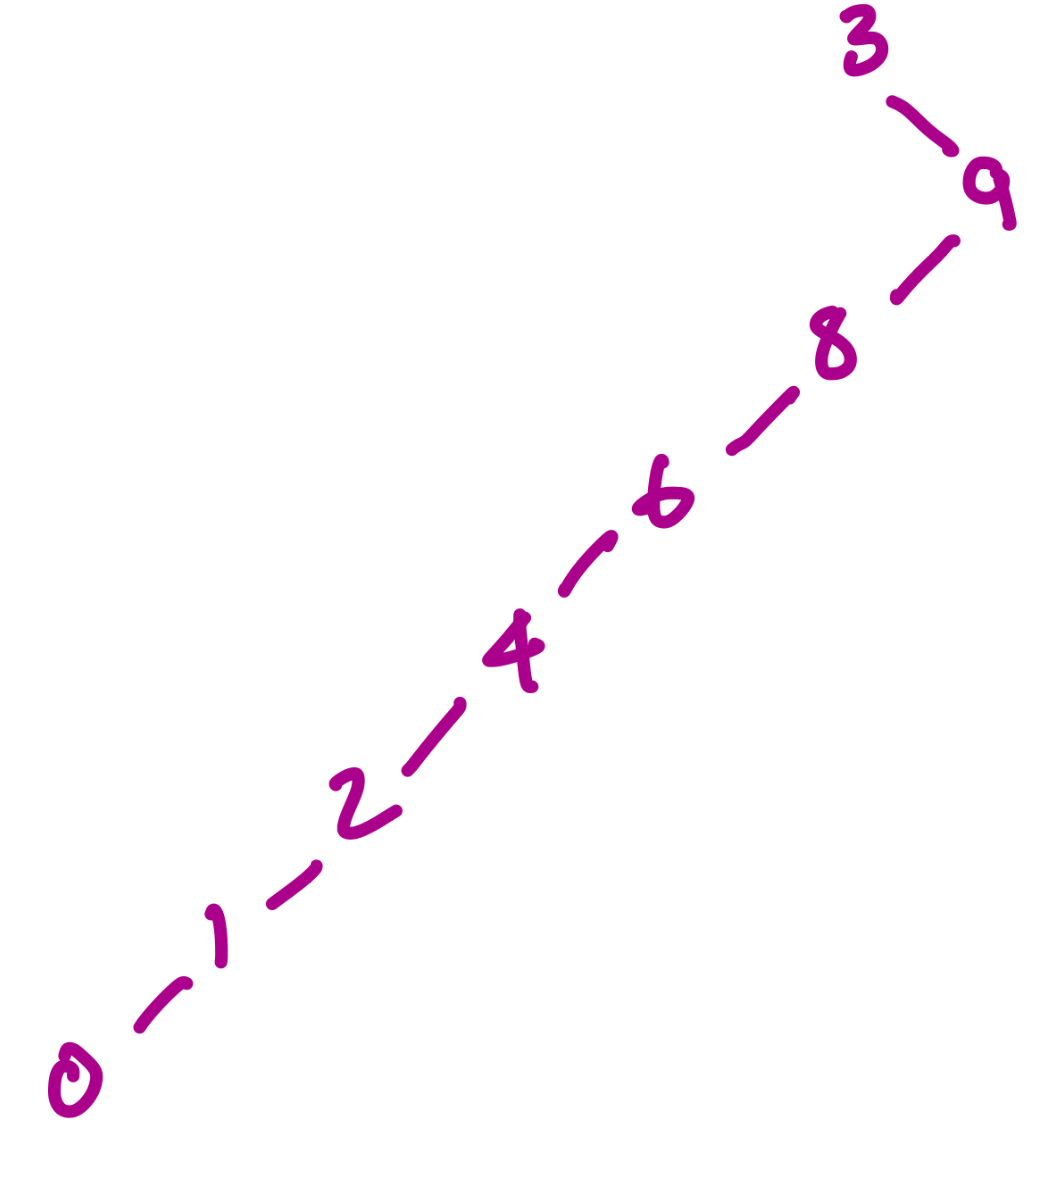
\includegraphics[width=0.3\textwidth]{3_5_removed.jpeg} \\
\end{tabular}

\begin{tabular}[t]{lcc}
  \textbf{insertion order} &  \textbf{tree from insertion} & \textbf{tree after removal of 5} \\
6 & 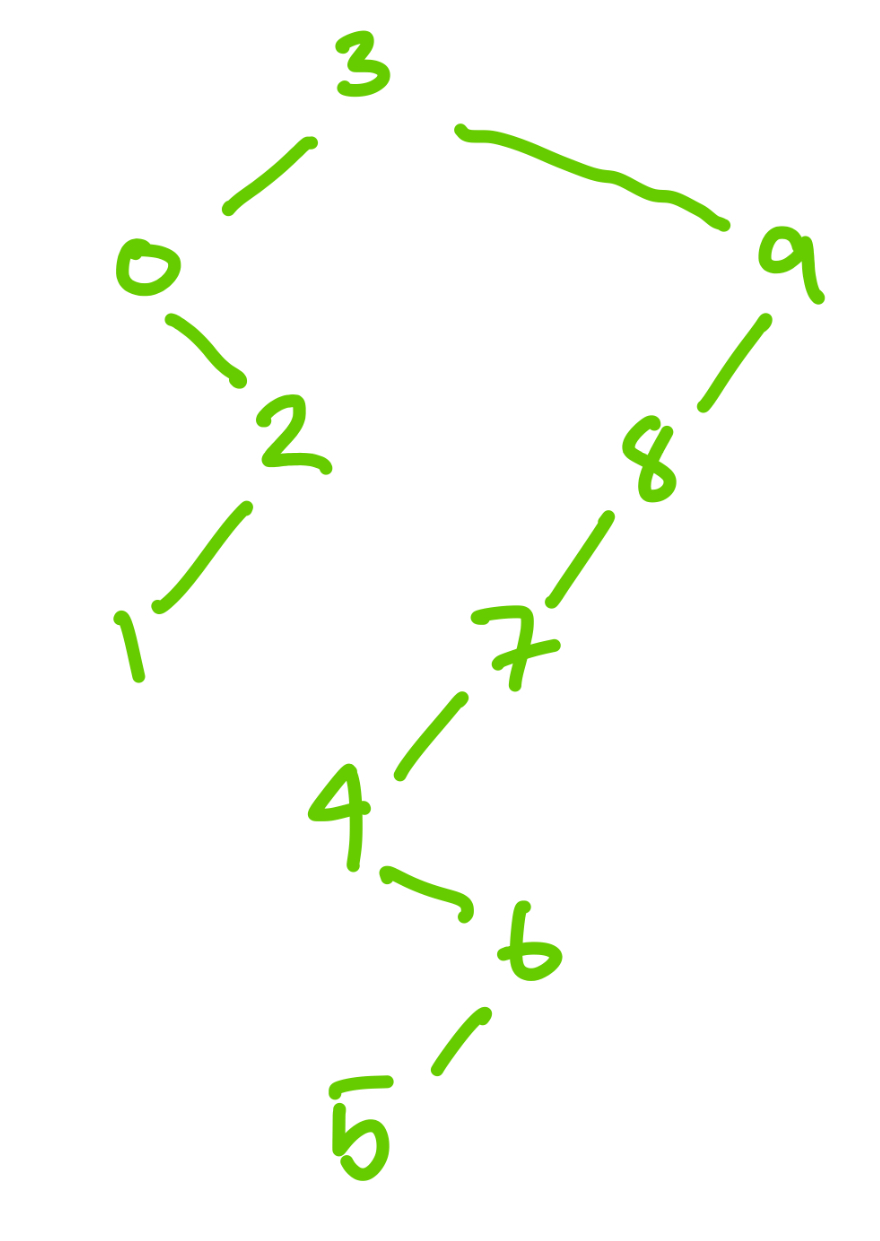
\includegraphics[width=0.3\textwidth]{3_6.jpeg} & 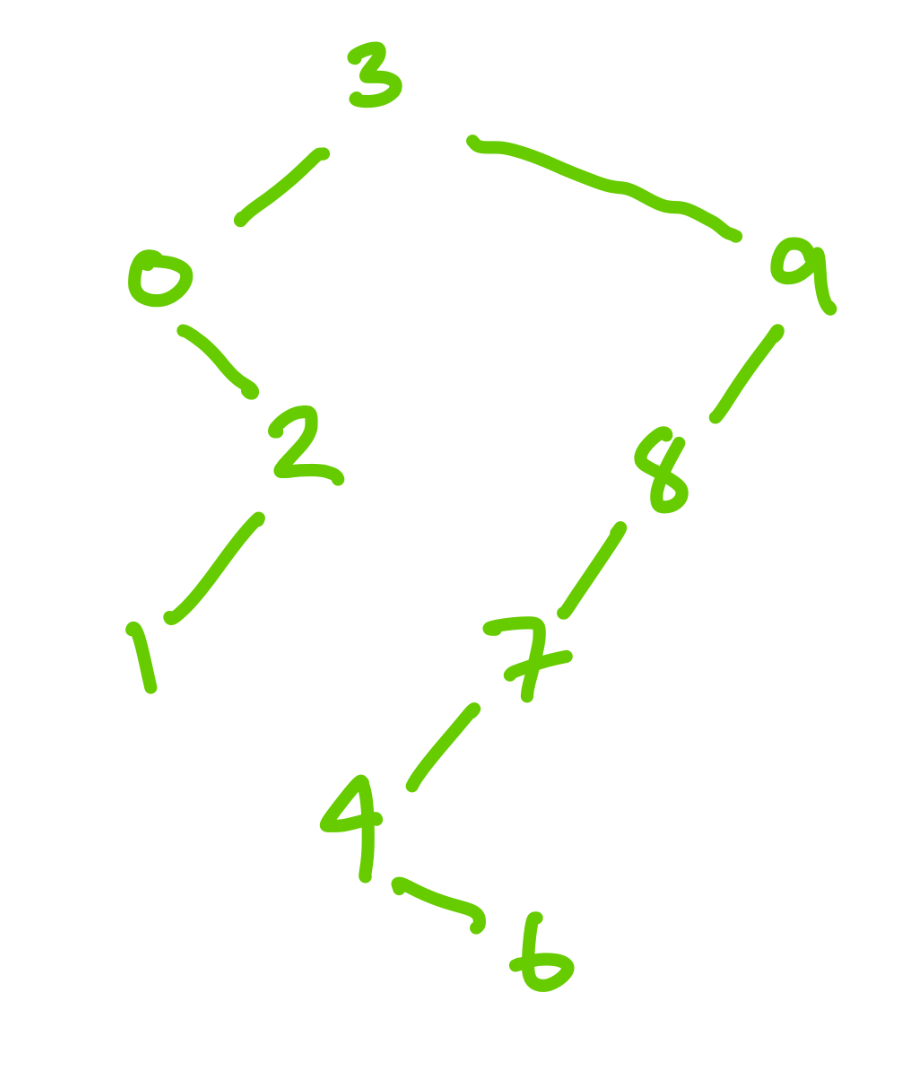
\includegraphics[width=0.3\textwidth]{3_6_removed.jpeg} \\
7 & 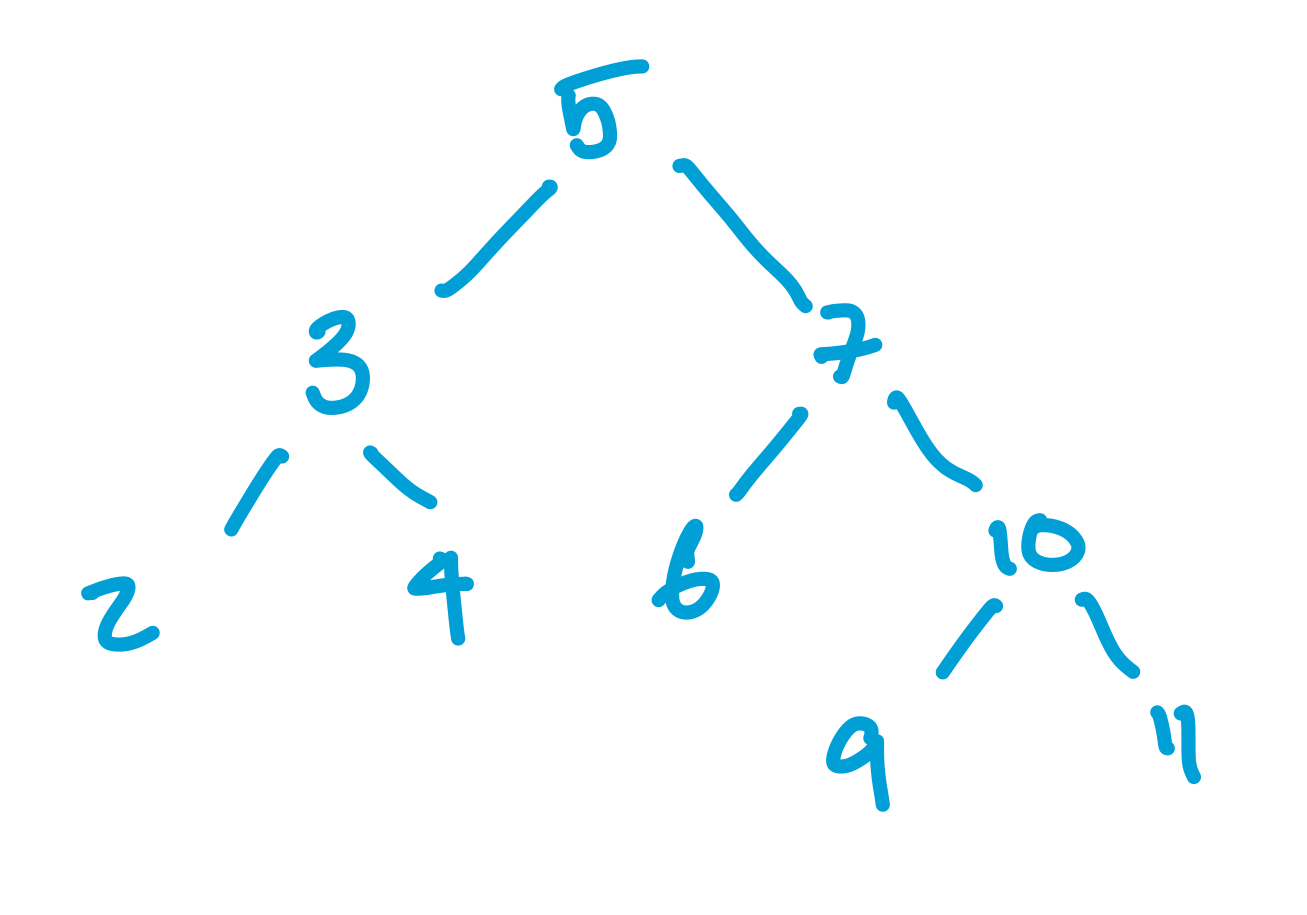
\includegraphics[width=0.3\textwidth]{3_7.jpeg} & 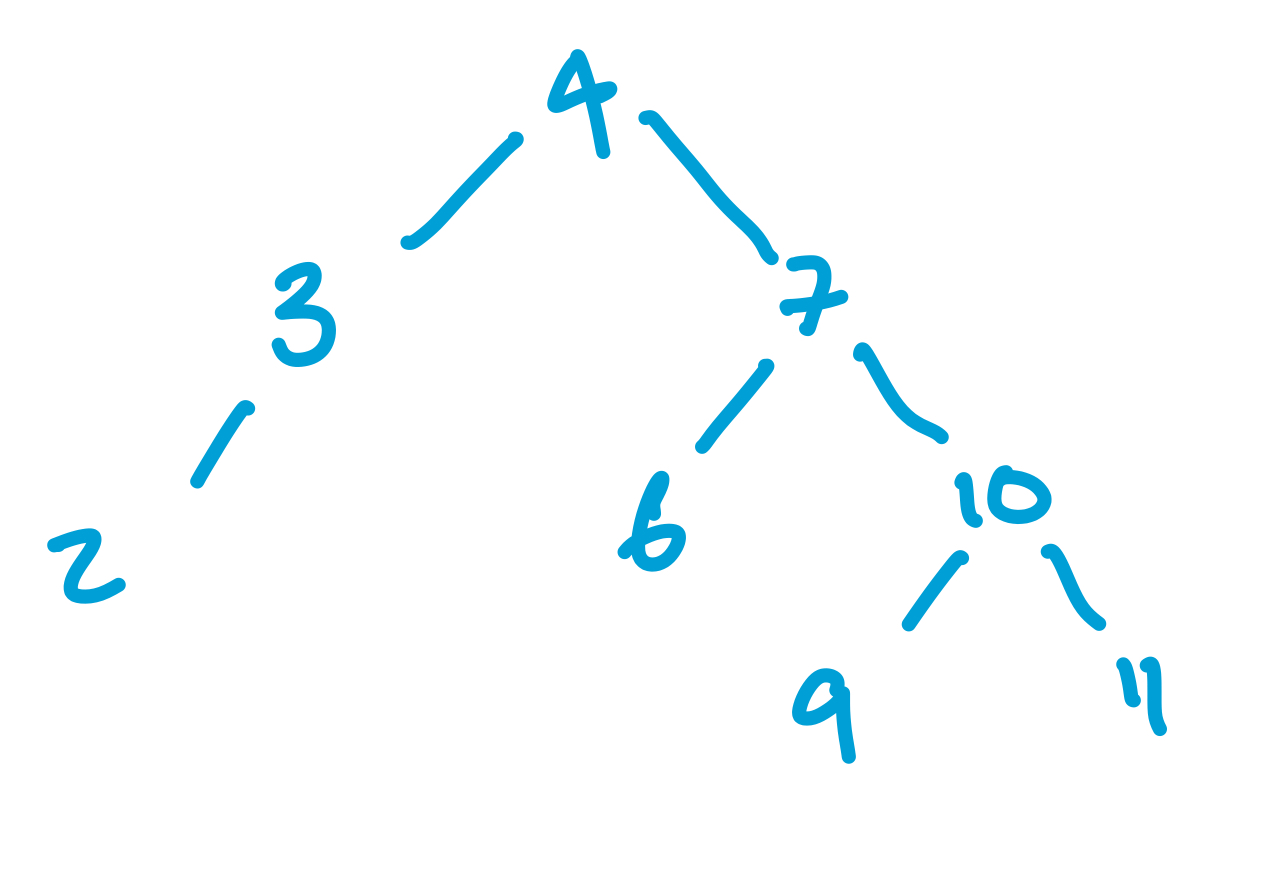
\includegraphics[width=0.3\textwidth]{3_7_removed.jpeg} \\
\end{tabular}
\end{document}